\section{Results}
\label{sec:results}

\subsection{Trial-vs-Subject CV Inflation}
\label{sec:results:cv}

Table~\ref{tab:cv-gap} reports balanced accuracy under both protocols on
UCSD Stress. All three FMs drop $\sim$21~points moving from trial-level to
subject-level evaluation. The gap is consistent across architectures.

\begin{table}[h]
\centering
\caption{Trial- vs.\ subject-level CV gap on UCSD Stress. Values are
recording-level balanced accuracy.}
\label{tab:cv-gap}
\small
\begin{tabular}{lccc}
\toprule
Model & Trial-level \BA{} & Subject-level \BA{} & Gap \\
\midrule
LaBraM   & 0.862 & 0.656 & $-20.6$ \\
REVE     & 0.770 & 0.553 & $-21.7$ \\
CBraMod  & 0.712 & 0.488 & $-22.4$ \\
\bottomrule
\end{tabular}
\end{table}

% TODO: add bootstrap CIs and a paired sign-test result over the 3 FMs.

\subsection{Frozen Feature Variance Decomposition}
\label{sec:results:eta}

Table~\ref{tab:eta} reports $\eta^{2}$ for subject and label factors on
frozen LaBraM features (19 common channels). Subject identity dominates
label signal by 11--13$\times$ when subject count is matched.

\begin{table}[h]
\centering
\caption{Variance decomposition of frozen LaBraM features.
$N$-matched ADFTD averages 10 random draws of 17 subjects.}
\label{tab:eta}
\small
\begin{tabular}{lrrrr}
\toprule
Dataset & $N_{\mathrm{subj}}$ & $\eta^{2}_{\mathrm{subj}}$ & $\eta^{2}_{\mathrm{label}}$ & Ratio \\
\midrule
UCSD Stress & 17 & 0.649 & 0.059 & 11.0 \\
ADFTD (full) & 65 & 0.783 & 0.024 & 33.0 \\
ADFTD ($N$-matched) & 17 & $0.748 \pm 0.042$ & $0.062 \pm 0.016$ & $13.0 \pm 3.9$ \\
\bottomrule
\end{tabular}
\end{table}

% TODO: add row for TDBRAIN once frozen-feature analysis is regenerated.
% TODO: add a permutation-test p-value column.

\subsection{Cross-Dataset Signal Strength}
\label{sec:results:cross}

Figure~\ref{fig:cross-dataset} compares fine-tuned LaBraM balanced accuracy
and frozen-vs-fine-tuned $\eta^{2}$ ratios across all three datasets. Three
patterns are visible.

First, recording-level \BA{} ranks the three datasets in the expected
direction: Stress at $0.656$, TDBRAIN at $0.681$, ADFTD at $0.752$. All are
above chance ($0.5$); the spread is $\sim$10 points.

Second, frozen $\eta^{2}$ ratios are uniformly large but not equal:
$10.0\times$ for Stress, $31.5\times$ for TDBRAIN, $33.0\times$ for ADFTD.
The latter two are larger because their subject pools are larger ($N{=}359$
and $N{=}65$ respectively), inflating the between-subject sum of squares.

Third --- and this is the central observation --- fine-tuning shifts the
$\eta^{2}$ ratio in opposite directions for ADFTD and TDBRAIN. For ADFTD,
the ratio drops from $33.0$ to $13.9$: fine-tuning amplifies label
information faster than it amplifies subject identity, consistent with a
strong, separable diagnostic signal. For TDBRAIN, the ratio rises from
$31.5$ to $64.4$: fine-tuning amplifies subject identity \emph{more} than
label information, consistent with the model fitting the
$\sim$$7{:}1$ class imbalance ($N_{\mathrm{MDD}}{=}640$,
$N_{\mathrm{HC}}{=}94$) by collapsing toward the majority class. For
Stress, the ratio is essentially flat ($10.0 \to 12.3$): there is too
little label variance for fine-tuning to amplify either direction.

\begin{figure}[h]
  \centering
  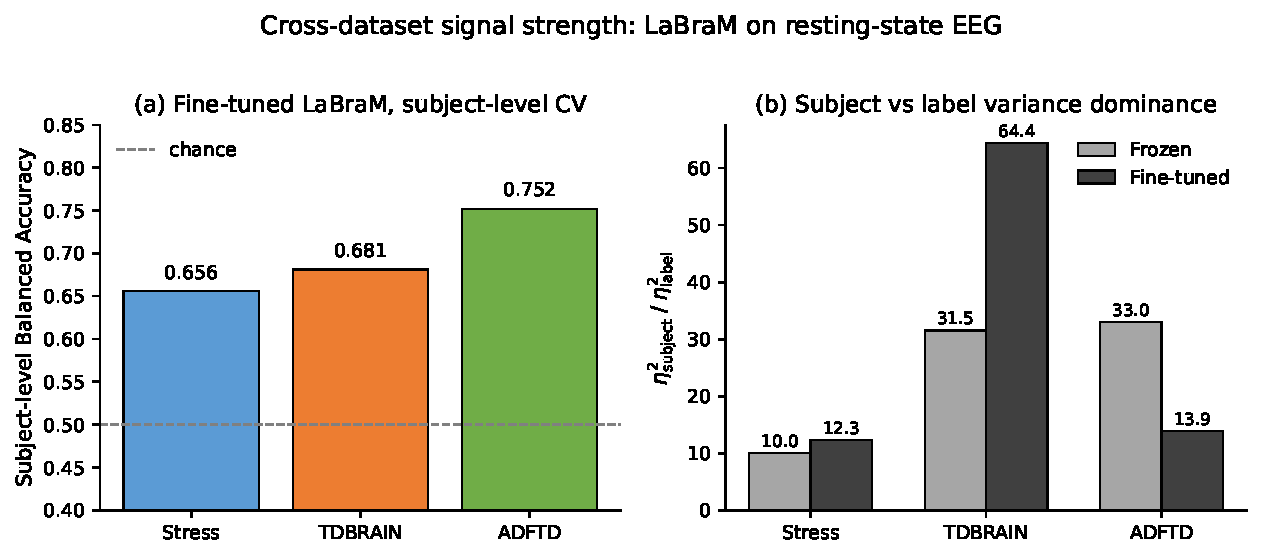
\includegraphics[width=0.95\linewidth]{figures/cross_dataset_signal_strength.pdf}
  \caption{Cross-dataset signal strength under LaBraM, subject-level
  5-fold CV. \textbf{(a)}~Recording-level balanced accuracy after full
  fine-tuning. All three datasets exceed chance, with a $\sim$10-point
  spread. \textbf{(b)}~$\eta^{2}_{\mathrm{subject}}/\eta^{2}_{\mathrm{label}}$
  ratio for frozen and fine-tuned features. ADFTD's ratio drops sharply
  with fine-tuning (label signal amplified); TDBRAIN's ratio rises
  (subject identity amplified due to class imbalance); Stress is flat
  (signal-limited at the source).}
  \label{fig:cross-dataset}
\end{figure}

\subsection{Frozen vs.\ Fine-Tuned $\eta^{2}$ Shift}
\label{sec:results:ft}

Table~\ref{tab:ft-shift} compares frozen and fine-tuned LaBraM features on
the two reference datasets. Fine-tuning increases both subject and label
encoding, but the ratio behaves differently: it drops sharply for
Alzheimer's ($13.0 \to 7.7$) and remains essentially flat for stress
($11.0 \to 12.8$). This is the central finding for our claim that
\textbf{fine-tuning cannot create signal that isn't in the raw EEG.}

\begin{table}[h]
\centering
\caption{Frozen vs.\ fine-tuned LaBraM features ($N=17$ matched).}
\label{tab:ft-shift}
\small
\begin{tabular}{llrrrr}
\toprule
Dataset & Mode & $\eta^{2}_{\mathrm{subj}}$ & $\eta^{2}_{\mathrm{label}}$ & Ratio & \BA{} \\
\midrule
Stress & Frozen & 0.649 & 0.059 & 11.0 & --- \\
Stress & FT     & 0.874 & 0.069 & 12.8 & 0.656 \\
\addlinespace
ADFTD ($N$-matched) & Frozen & 0.748 & 0.062 & 13.0 & --- \\
ADFTD ($N$-matched) & FT     & 0.930 & 0.125 & 7.7  & 0.752 \\
\bottomrule
\end{tabular}
\end{table}

\subsection{Classical Baseline Parity}
\label{sec:results:classical}

Table~\ref{tab:classical} compares classical hand-crafted features
(absolute and relative band power, frontal asymmetry, ratios) against
fine-tuned LaBraM under identical subject-level CV. Random forest matches
or slightly exceeds LaBraM on both datasets.

\begin{table}[h]
\centering
\caption{Classical features vs.\ fine-tuned LaBraM, subject-level 5-fold
CV. \BA{} reported.}
\label{tab:classical}
\small
\begin{tabular}{lcc}
\toprule
Method & Stress \BA{} (70-rec) & ADFTD \BA{} \\
\midrule
LaBraM (FT)            & 0.656 & 0.752 \\
RF on band power (full ch) & \textbf{0.666} & \textbf{0.753} \\
RF on band power (19 ch) & 0.536 & 0.753 \\
LogReg (L2)            & 0.624 & --- \\
SVM (RBF)              & 0.580 & --- \\
\bottomrule
\end{tabular}
\end{table}

\subsection{Failed Mitigation: Subject-Adversarial Training}
\label{sec:results:adv}

We implemented subject-adversarial training via gradient reversal layer
(GRL) and a LEAD-style auxiliary subject classification loss. Neither
improves performance; both degrade it
(Table~\ref{tab:adv}). We treat this as evidence that the diagnostic
signal in resting-state stress is not amplifiable by removing subject
information --- it is signal-limited at the source.

\begin{table}[h]
\centering
\caption{Failed mitigation strategies on UCSD Stress. \BA{} subject-level
5-fold CV.}
\label{tab:adv}
\small
\begin{tabular}{lc}
\toprule
Method & Stress \BA{} \\
\midrule
LaBraM FT (baseline) & 0.656 \\
+ GRL ($\lambda{=}0.05$) & 0.537 \\
+ LEAD subject loss     & 0.439 \\
GRL $\lambda$ sweep $\{0.01,0.05,0.1,0.5,1.0\}$ & all $<$ baseline \\
\bottomrule
\end{tabular}
\end{table}

% TODO: add §6.2 spectral-guided FiLM conditioning (pending experiment).
